\chapter{Document Finder}\label{chap:finder}

Most new students of Pāli or Buddhism are not familiar with the structure of the Pāli canon. Finding a document by navigating TOC Tree can be difficult. That is why Document Finder comes in. This tool is part of the tab area in the main window. It can also be opened as a separate window by {\faSix \symbol{"F002}} button, or menu Reader > {\faSix \symbol{"F002}} Document Finder.

A simple use of this tool is you can see all texts in a selected collection. The tabular display of the result can make the navigation easier. You can also narrow down the scope of selection by choosing a suitable text group using its dropdown option (see Figure \ref{fig:finder-textgroup}). The available text groups are preset according to the arrangement of the corpus.\footnote{It is impossible to add a specific text group by the user. If that kind of group is really needed for a specific purpose, please send a request to the author.}

\begin{figure}[!hbt]
\centering
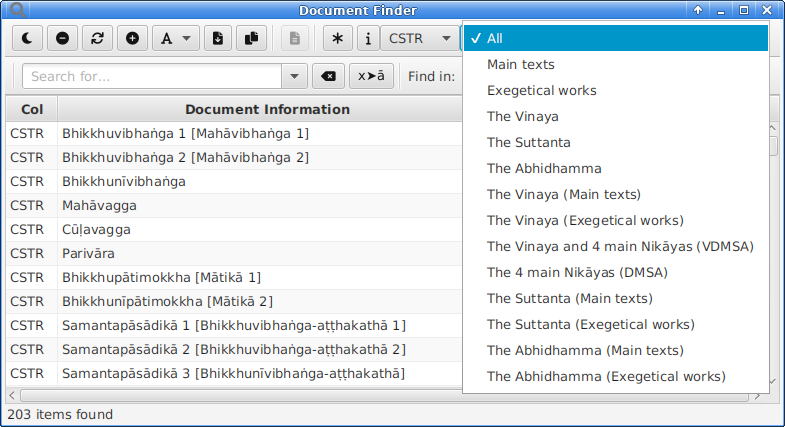
\includegraphics[width=0.9\linewidth]{images/finder-textgroup.png}\\
\caption{Text group selector in Document Finder}
\label{fig:finder-textgroup}
\end{figure}

If you have some information about the document you are looking for, you can filter the result by entering a query in the search box. There are three modes of search: (1) search in document information, (2) search in document references, and (3) search in the content of documents. You have to select a suitable mode first.

\section{Filtering by document information}

\begin{figure}[!hbt]
\centering
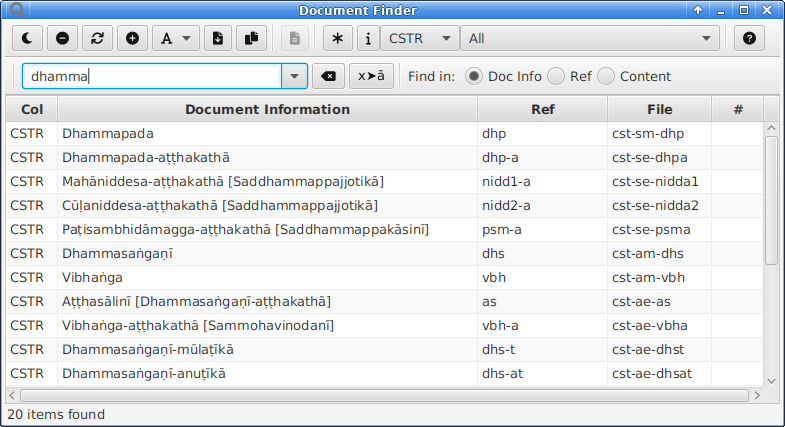
\includegraphics[width=0.9\linewidth]{images/finder-infosearch.png}\\
\caption{Filtering by searching in document information}
\label{fig:finder-infosearch}
\end{figure}

The simplest filtering is that of document information search, as shown in Figure \ref{fig:finder-infosearch}. Document information consists of text title, description, and other additional fields that are predefined for each collection (some collections may have little information to search). As you can see in the result exemplified, the query `dhamma' may match several fields, not only the title of documents. This can be alternative titles, as shown in brackets; or description, not shown in the table, by which the query word is not visible in the entries. This filtering mode is quite useful when searching in all collections, enabled by {\faSix \symbol{"F069}} button (see box note below).

\dothis{If you want to show all documents in all collections at once, use {\faSix \symbol{"F069}} toggle button.}

\section{Filtering by references}

If you do a lot of academic writing, you may need to find a document by its reference. This task is in fact very difficult (to nearly impossible). At best, we can do just showing documents that may be related \emph{somehow} with a specific reference. The `somehow' stressed here tells us that sometimes the result often comes with a surprise because the query may match some other criterion unexpected to the user.

\begin{figure}[!hbt]
\centering
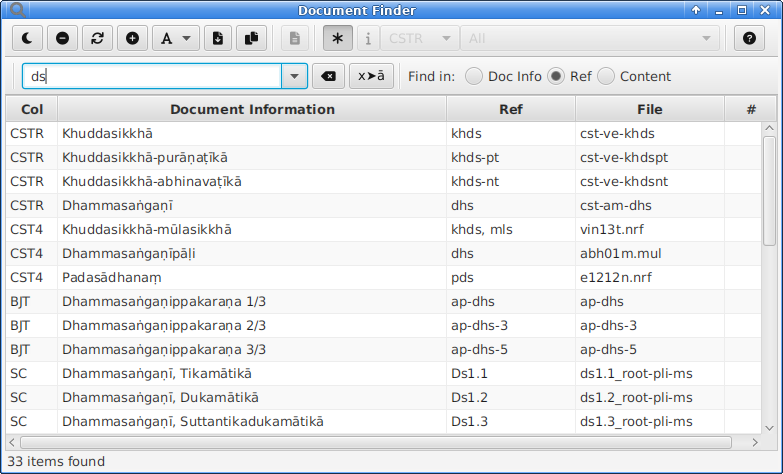
\includegraphics[width=0.9\linewidth]{images/finder-refsearch.png}\\
\caption{Filtering by searching in references}
\label{fig:finder-refsearch}
\end{figure}

Figure \ref{fig:finder-refsearch} shows a filtering result by references with `ds' (perhaps you have Dhammasaṅgaṇī in mind) in all collections. As you can see, apart from Dhammasaṅgaṇī in SuttaCentral that use `ds' as its reference, the similar results from other collections also show up even though they use a different reference for this book, e.g., `dhs.' Moreover, references that can match with this query somehow are also listed together. You may count these as noise. But if you do not have Dhammasaṅgaṇī in mind, the document you are looking for may be one of this noise.

\dothis{To see the reference table of all documents, select menu Reader > {\faSix \symbol{"F00A}} Reference Table.}

To help students tackle with the headache of Pāli text referencing, \emph{Reference Table} is added to \textsc{Pāli\,Platform\,3}. This tool shows all references used in all collections, together with those used by academics. You can do a simple search in this table to filter what you are interested in. See Figure \ref{fig:reference-table} in comparison with the result from reference filtering above.

\begin{figure}[!hbt]
\centering
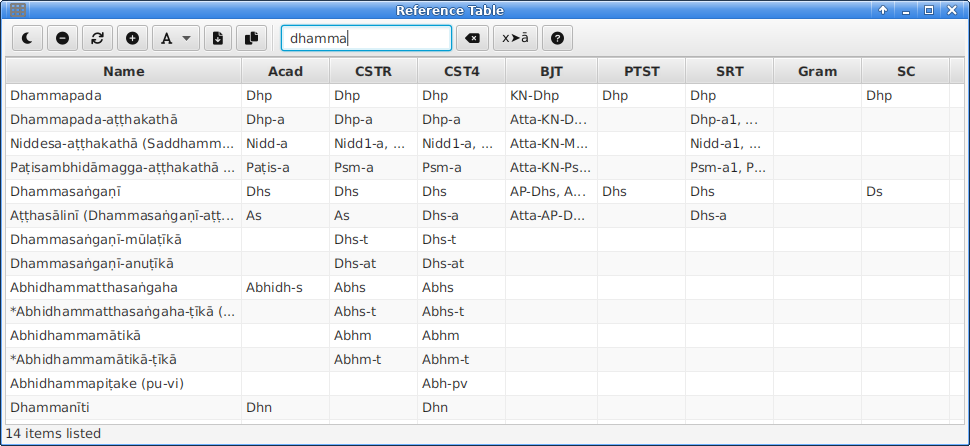
\includegraphics[width=0.9\linewidth]{images/reference-table.png}\\
\caption{Reference Table}
\label{fig:reference-table}
\end{figure}

\section{Filtering by content search}

If the two filtering modes above cannot bring you the right result, or you just have a portion of text to search, the last resort in this tool is content search. In this mode the query is always treated as regular expression, and you have to hit the Enter key to trigger the search, except when switching from other modes. When some text is found, the last column of the result shows the number of hits in the document. Figure \ref{fig:finder-contentsearch} shows the result of an attempt to find \pali{Dhammacakkappavattanasutta} with pattern `\texttt{$\backslash$b[dD]hammacakkappa.*$\backslash$b}'.

\boxnote{The pattern `\texttt{$\backslash$b[dD]hammacakkappa.*$\backslash$b}' explained (for more information on regular expression see Chapter \ref{chap:regexp}):\\
\hspace{5mm}\bullet\ \textbf{$\backslash$b} marks the word boundary, meaning the word has to stand by its own, not within a compound.\\
\hspace{5mm}\bullet\ \textbf{[dD]} allows either `d' or `D' to be matched. This can cover capitalized cases.\\
\hspace{5mm}\bullet\ \textbf{hammacakkappa} is an exact sequence to be matched.\\
\hspace{5mm}\bullet\ \textbf{.*} means any number of characters (including zero) following that sequence.
}

Remember that this full-text search is case sensitive (making your search query precise can narrow down the result significantly), and brute (it searches directly in all files one by one, and you have to wait until it finishes). Since complex patterns take more time to process, it is better to use an exact query rather than meta-characters if you have those in mind. If the search fails after all, consider using a more sophisticated tool, such as Lucene Finder (see Chapter \ref{chap:lucene}).

\begin{figure}[!hbt]
\centering
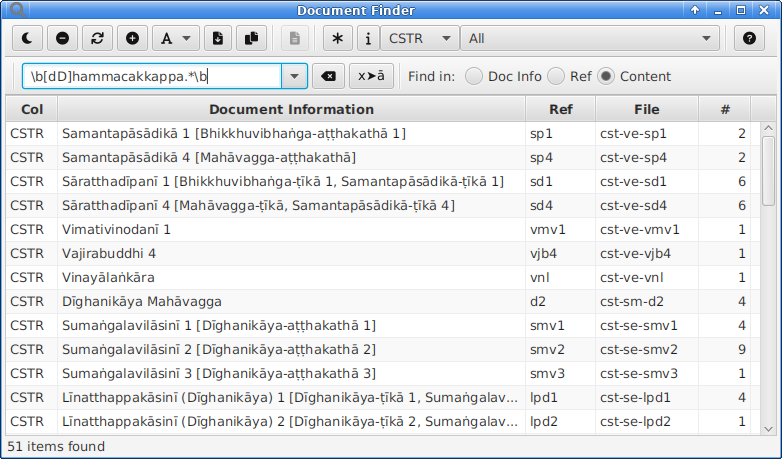
\includegraphics[width=0.9\linewidth]{images/finder-contentsearch.png}\\
\caption{Filtering by searching in content}
\label{fig:finder-contentsearch}
\end{figure}

\boxnote{Content search is brute and slow, and it is likely to fail in structured documents like XML if the word you are looking for sits across tags. So, it should be used with a single-term search (yet, the target result can be missed).\\
\caveat{Avoid doing the content search with all collections at once by a complex pattern. This may paralyze the tool. Try selecting only one collection, or better only one text group, first.}
}

